\chapter{2010}
\label{cha:2010}

\begin{Problema}{1}
  Se tiene una hoja de papel de forma rectangular con v\'ertices
  $ABCD$ (ver figura). El lado de enfrente es azul y el de atr\'as
  blanco. Se toma la esquina $B$ y se dobla la hoja a lo largo de la
  l\'inea punteada $AF$ de tal forma que el lado $AB$ quede sobre el
  lado $AD$ y la esquina $B$ sobre el punto $E$. Luego se dobla la
  esquina $D$ de forma que el segmento ED quede sobre el segmento
  $EF$. Si el lado $AB$ mide $13$ cent\'imetros y el lado $BC$ mide
  $19$ cent\'imetros, calcula el \'area azul que queda descubierta.

  \begin{center}
    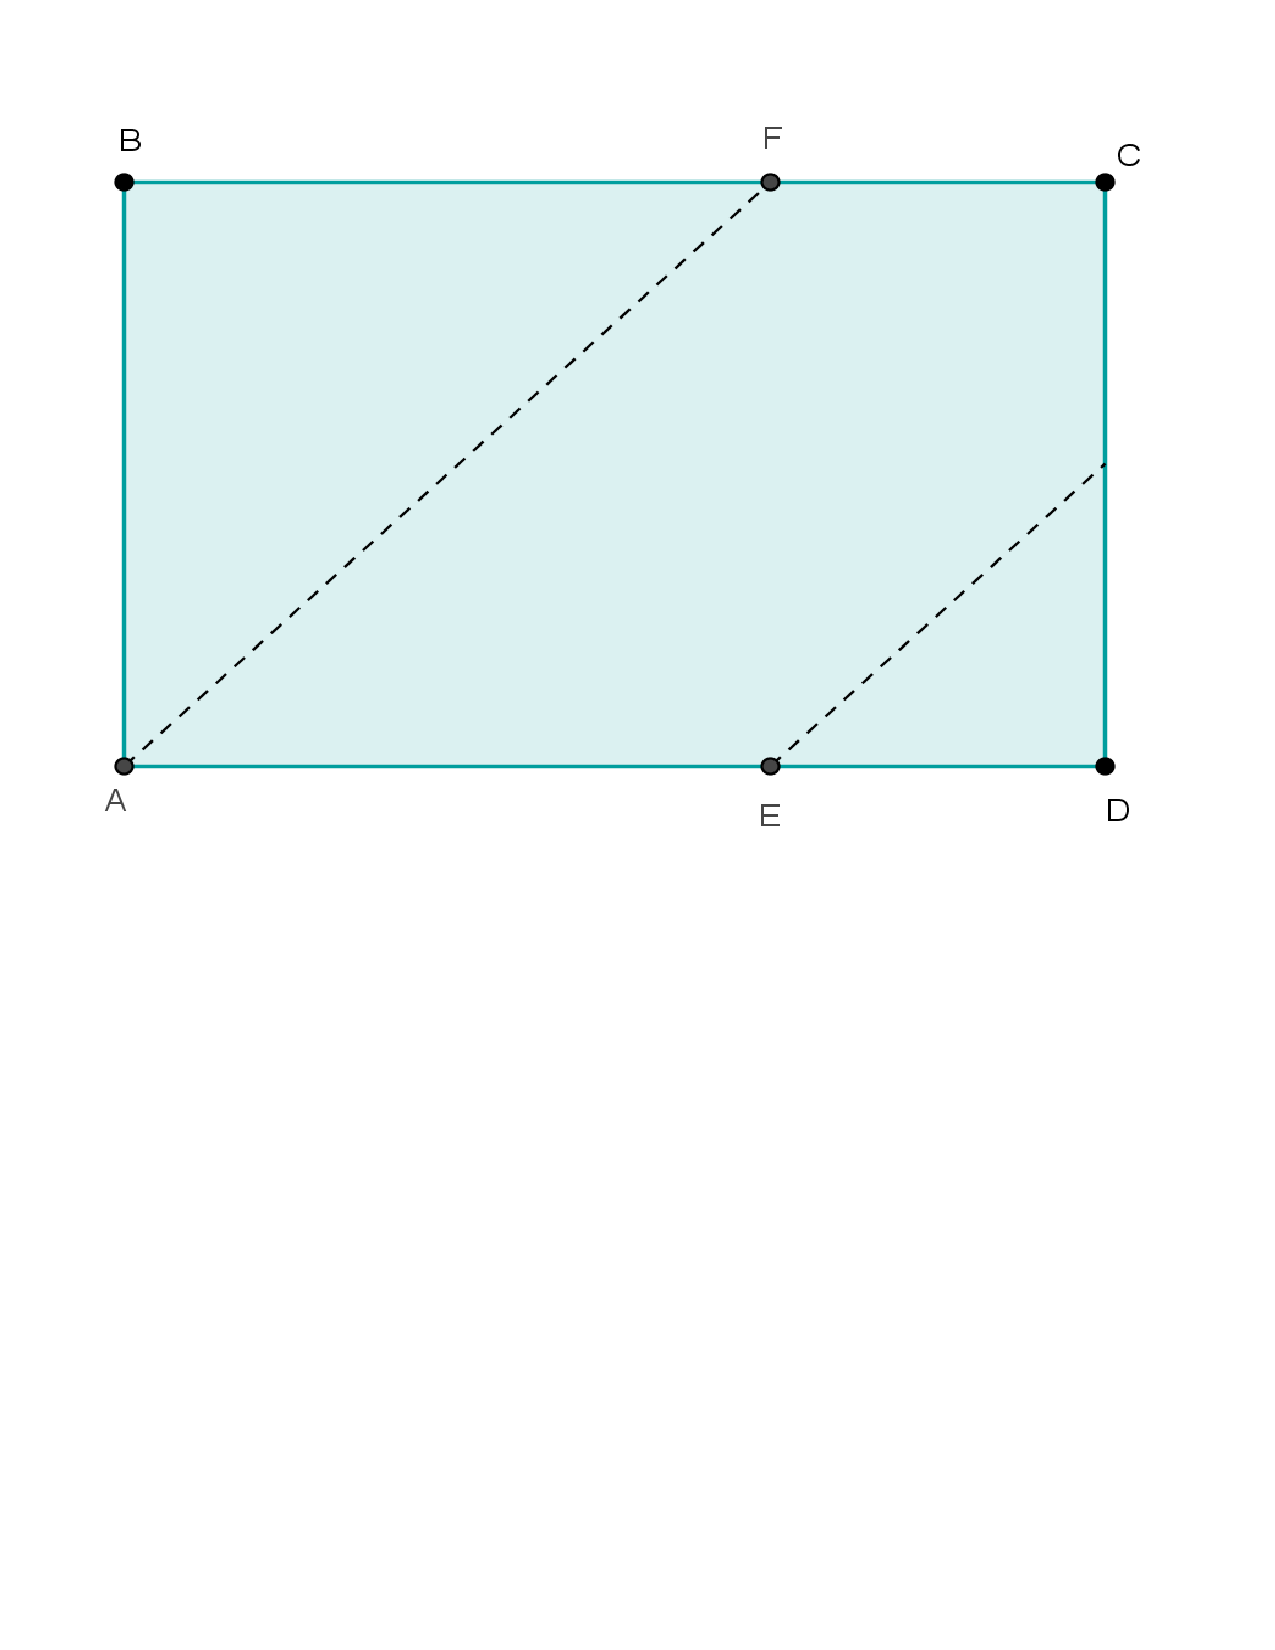
\includegraphics[scale=0.5,viewport=13 358 569 764]{hoja1.pdf}
  \end{center}
\end{Problema}

\begin{Solucion}
  
\end{Solucion}

\begin{Problema}{2}
  Un granjero compr\'o $100$ animales por $420,000$ pesos. Compr\'o
  vacas, borregos y cerdos. Cada vaca le cost\'o $5,000$ pesos, cada
  borrego $4,000$ pesos y cada cerdo $3,000$ pesos. ?`De cu\'antas
  maneras distintas pudo haber comprado estos animales, si sabemos que
  compr\'o al menos 10 de cada especie?
\end{Problema}

\begin{Solucion}
  
\end{Solucion}

\begin{Problema}{3}
  Un cient\'ifico ha inventado una m\'aquina del tiempo. Esta
  m\'aquina tiene la peculiaridad que solamente puede viajar en
  periodos de $1971$ a\~nos hacia el futuro y $2010$ a\~nos hacia el
  pasado. ?`Cu\'antos viajes hacia el futuro y cu\'antos viajes al
  pasado deben hacerse con esa m\'aquina para avanzar exactamente $3$
  a\~nos al futuro?
\end{Problema}

\begin{Solucion}
  
\end{Solucion}

\begin{Problema}{4}
  Juanita est\'a intentando accesar una de sus cuentas de correo, pero
  olvid\'o su contrase\~na. Lo \'unico que recuerda es que su
  contrase\~na es de 10 caracteres y estos son los mismos que los de
  la palabra MATEMATICA, pero no recuerda en qu\'e orden. Por ejemplo,
  la contrase\~na podr\'ia ser CAAMETIAMT. ?`Cu\'antas diferentes
  posibilidades hay para su contrase\~na?
\end{Problema}

\begin{Solucion}
  
\end{Solucion}

\begin{Problema}{5}
  Considera la suma
  $$
  (1 \times 1!) + (2 \times 2!) + (3 \times 3!) +  \cdots + (2010 \times 2010!),
  $$ 
  donde los puntos suspensivos representan los t\'erminos
  intermedios. Demuestra que la suma es igual a $k!-1$ para alg\'un
  entero positivo $k$ y encuentra el valor de $k$.

  {\sl El s\'imbolo $n!$ significa el producto de los enteros
    positivos de $1$ hasta $n$. Por ejemplo,
    $$
    5!=1\times 2  \times 3 \times 4 \times 5=120.
    $$}
\end{Problema}

\begin{Solucion}
  
\end{Solucion}

\begin{Problema}{6}
  Considera el tri\'angulo $ABC$ y un punto $D$ sobre el lado
  $BC$. Sean $E$, $F$, $G$ y $H$ puntos medios de los segmentos $CD$,
  $DB$, $AC$ y $AB$, respectivamente. Muestra que el cuadril\'atero
  $EGHF$ es un paralelogramo y que su \'area es la mitad del \'area
  del tri\'angulo $ABC$.

  \begin{center}
    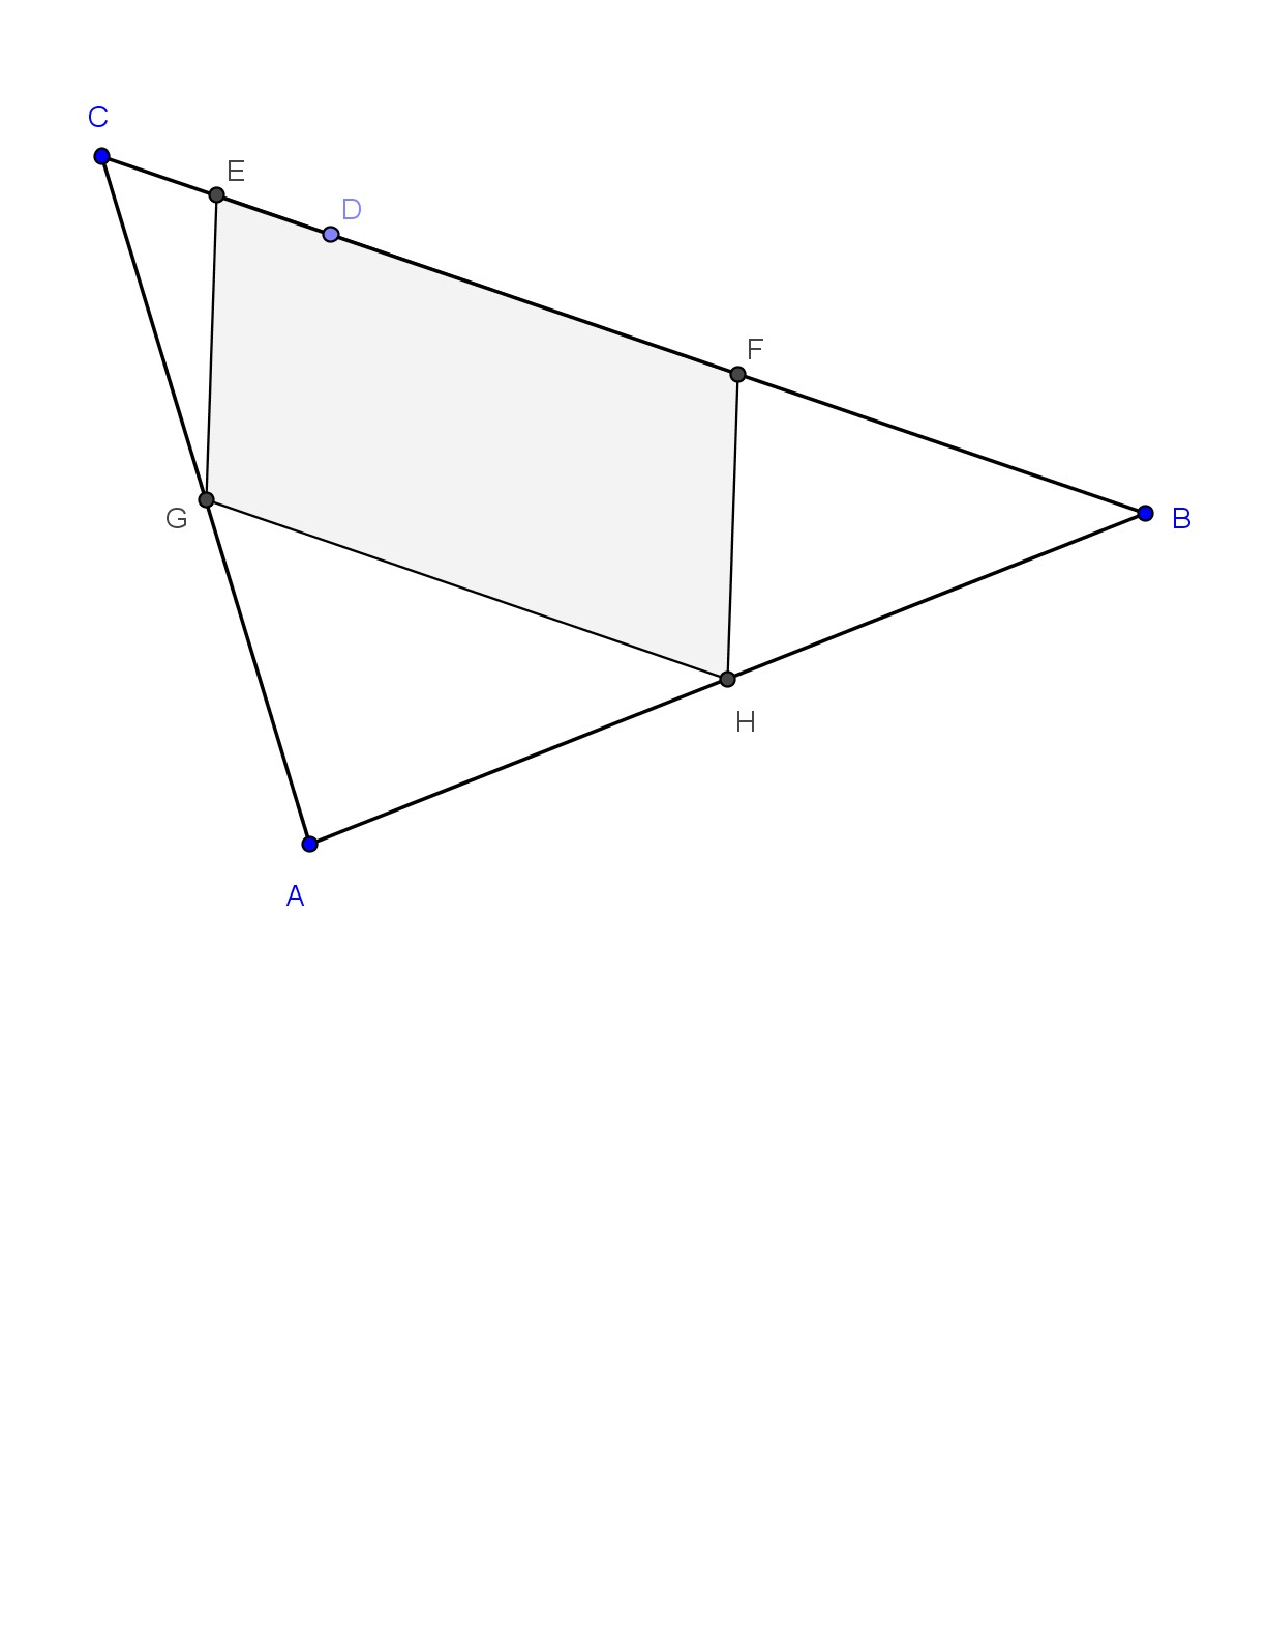
\includegraphics[scale=0.5,viewport=28 349 587 763]{Triangulo1.pdf}
  \end{center}
\end{Problema}

\begin{Solucion}
  
\end{Solucion}

%%% Local Variables: 
%%% mode: latex
%%% TeX-master: "libro"
%%% End: 